\chapter{Introduction}\label{ch:intro}

\section{The Nuclear Fuel Cycle}

The nuclear fuel cycle, in general, can be described as a set of facilities that
interact with one another to either provide or consume fuel services. The
overall goal of the nuclear fuel cycle is to provide fuel to nuclear power
plants which, in turn, generate energy. The overall goal of the system is to
produce power at a competitive price while managing externalities of the
process, the chief of which is spent nuclear fuel. There exist a myriad of
strategies to achieve this aim which generally fall along a spectrum of the
degree to which fuel is recycled. In general, fuel cycles on the end of the
spectrum that does not recycle fuel are concerned most with cost, whereas fuel
cycles that fully recycle fuel are concerned most with issues of sustainability
and intergenerational equity.

\subsection{The Open Fuel Cycle}
The open, or once-through, fuel cycle is relatively simple and is in place in
most countries in the world that currently utilize nuclear power. In practice,
the primary fuel element used in this type of cycle is uranium; however,
processed fertile material, such as thorium, can also be used. The fuel cycle is
considered open because fuel that is used in a reactor is stored indefinitely
once its reactivity has dropped below useful levels.

Beginning the fuel cycle process, uranium ore is initially extracted from the
ground using one of a variety of techniques including open pit mining,
underground mining, and \textit{in situ} leaching. The uranium ore is then
milled to form yellowcake, $\mathrm{U_3O_8}$. The tailings, or byproducts, of
this process are slightly radioactive and are therefore considered to be
low-level waste (LLW) by the Nuclear Regulatory Commission (NRC)
(see \cite{nrc_10_1985}).

Certain reactors are designed to use naturally enriched uranium. For these
reactors, yellowcake can be directly reduced with oxygen to form naturally
enriched uranium oxide, $\mathrm{UO_2}$. For the majority of power reactors,
however, the uranium must be enriched with higher-than-natural levels of
uranium-235. In order to do so, yellowcake is sent to a conversion facility,
which converts it from $\mathrm{U_3O_8}$ to $\mathrm{UF_6}$. The uranium
hexafluoride is then enriched to the required level in an enrichment facility,
of which three classes exist: gaseous diffusion, the original enrichment
technology; centrifugal diffusion, the current enrichment technology; and Atomic
Vapor Laser Isotope Separation (AVLIS), a newer technology not currently in
commercial production. The enriched uranium hexafluoride is then sent to a fuel
fabrication facility where it is returned to yellowcake form before being
reduced to uranium oxide. The uranium oxide is then sintered into pellets and
loaded into fuel assemblies to be placed in a reactor. This process, in
conjunction with uranium mining, is termed the \textit{front end} of the nuclear
fuel cycle.

Once fuel has been processed in a reactor, it is cooled off in pools for a
number of years, and then stored in dry casks before eventually being sent to a
final repository. The physical location of the fuel may vary during dry cask
storage between the reactor site or some other interim storage site.

Graphically, the open fuel cycle is shown in Figure \ref{fig:open-cycle}.

\begin{figure}[]
  \begin{center}
    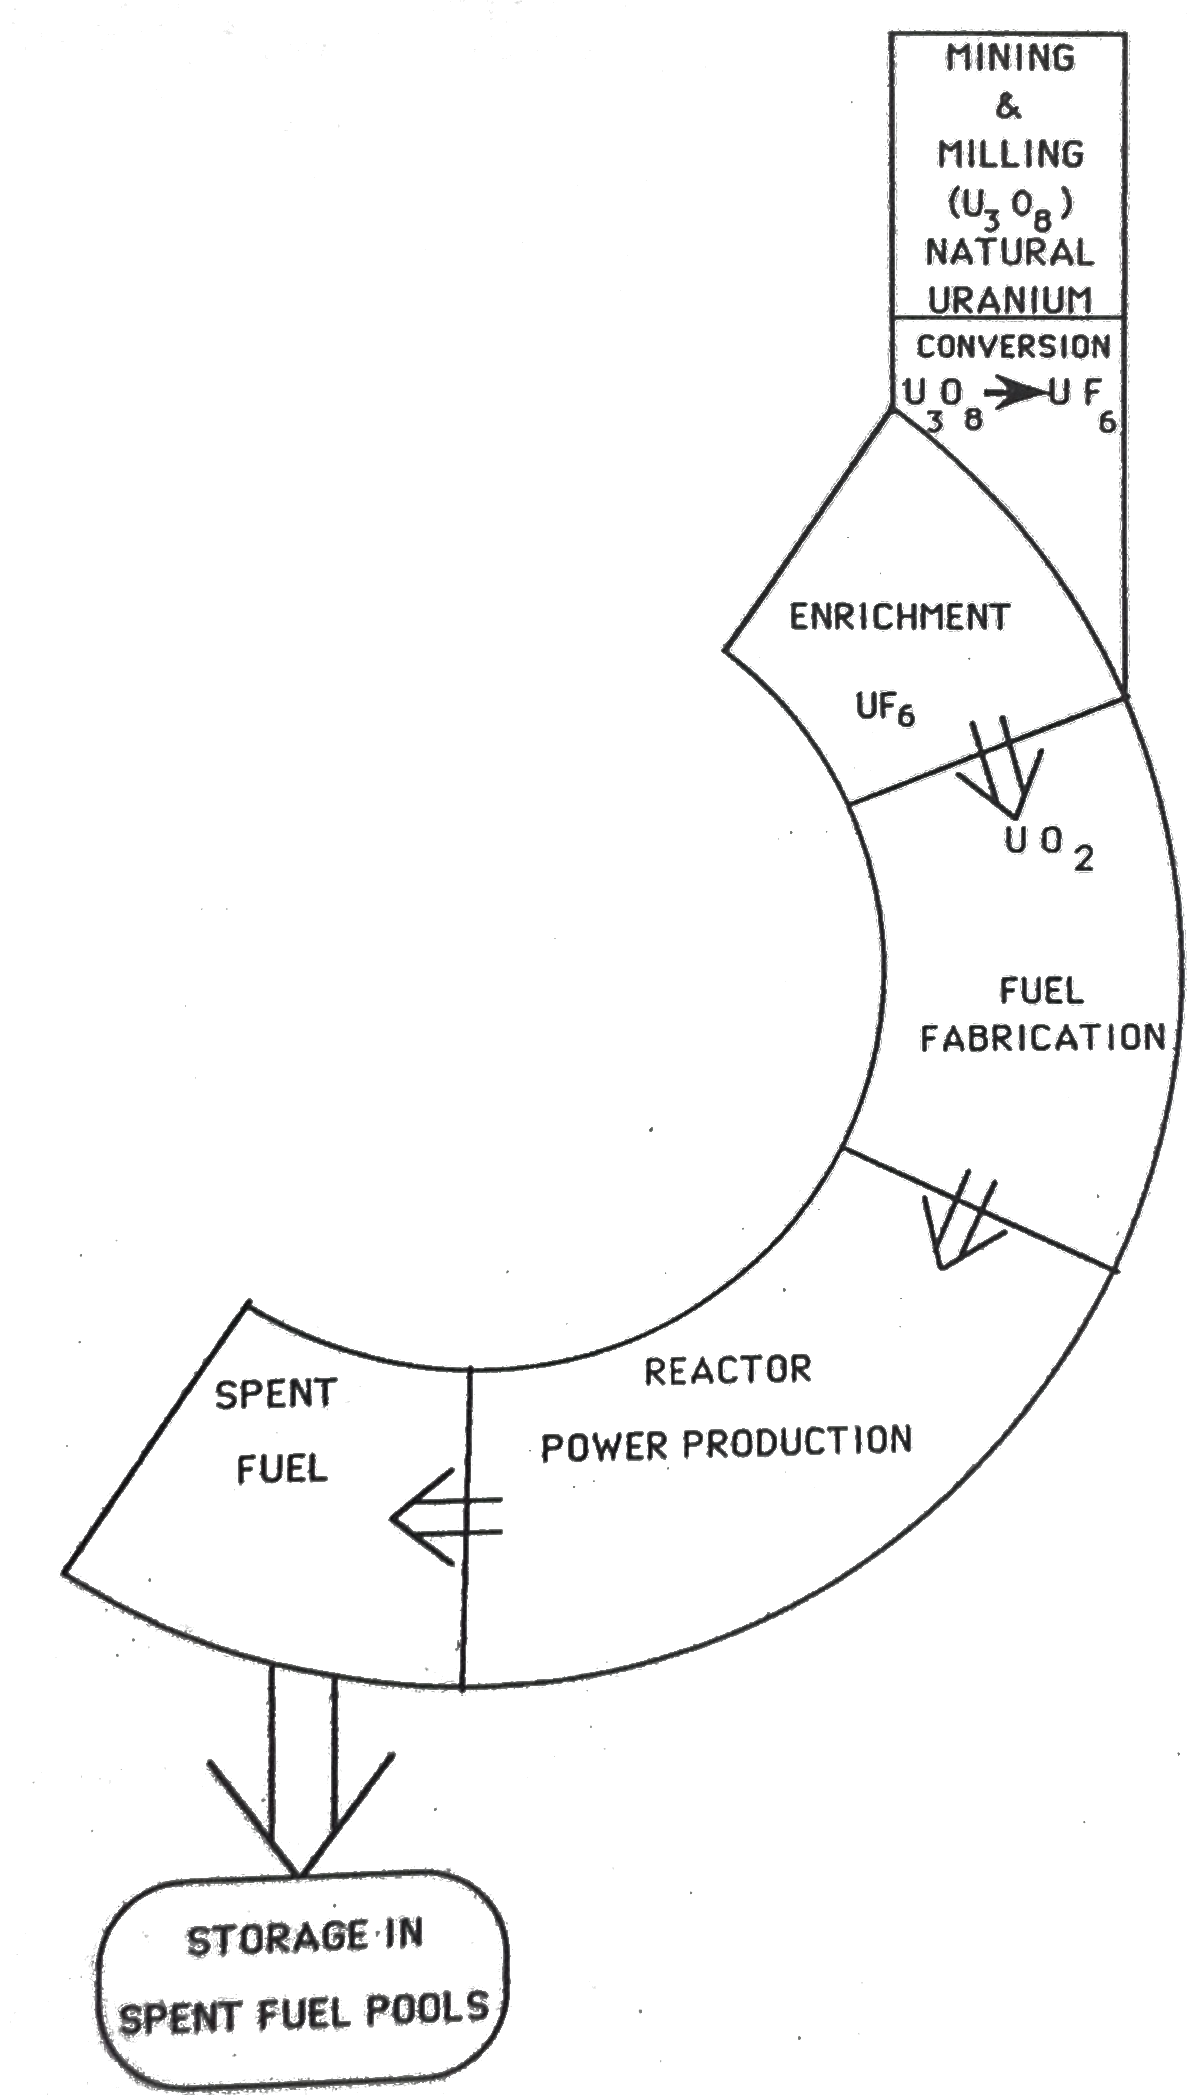
\includegraphics[height=7.5cm]{./chapters/intro/open_cycle.png}
  \caption{The once-through fuel cycle as shown in \cite{cochran1990nuclear}.}
  \label{fig:open-cycle}
  \end{center}
\end{figure}


\subsection{The Closed Fuel Cycle}
The closed fuel cycle is one that includes the recycling of used, or spent, fuel
to be reused in a reactor. Recycling used nuclear fuel is expensive due to the
costs associated with handling highly radioactive material (e.g., capital costs
of hot cells, etc.). However, there are at least two overarching benefits that
contribute to lowering the overall cost of the fuel cycle: increasing repository
capacity and increasing fuel utilization.

Spent fuel that exists the average Light Water Reactor (LWR) has an average
elemental makeup shown in Table \ref{tab:lwr_fuel}. Of the elements that
comprise used fuel, uranium, plutonium, and the mixed actinides (MA) are all
capable of producing power through the fission process. The fission products,
however, contain isotopes with high neutron capture cross sections, which
therefore act as poisons to the nuclear chain reaction. Achieving theoretical
100\% fuel utilization would thus require storing indefinitely only the fission
products and any other byproducts of the fuel cycle. Furthermore, repository
capacity is determined not only by total mass or volume, but also by heat load
and radiotoxicity, making the concentration of high-activity isotopes one of the
limiting factors in a repository's capacity. Fission products are generally
short-lived (in comparison to transuranic elements, i.e., uranium, plutonium,
and the MAs). Accordingly, by minimizing the amount of transuranics in a
repository, its capacity can be extended.

\begin{table} [h]
\centering
\begin{tabular} {|c|c|} 
\hline
Element Group & wt \% \\
\hline
Uranium           & $\sim$95  \\
Plutonium         & $\sim$1   \\
Mixed Actinides   & $\sim$0.1 \\
Fission Products  & $\sim$4   \\
\hline
\end{tabular}
\caption{Elemental Breakdown of Spent Fuel Exiting a Typical LWR}
\label{tab:lwr_fuel}
\end{table}

The act of reprocessing spent fuel is comprised of a number of
subprocesses. Once fuel has left the reactor core, it is stored in a spent fuel
pool for a some number of years, typically around five, in order to provide
enough time to lower decay heat to acceptable levels for handling of the
fuel. It can then be directly sent to a reprocessing facility or be sent for
some period of time to dry-cask storage. Reprocessing nuclear fuel is a chemical
extraction process and therefore is limited by chemical extraction
techniques. In general, there are two types of such processes: low-temperature
methods using organic solvents (e.g., PUREX), and high-temperature methods using
molten salts and metals, called pyroprocessing. The extraction techniques
separate the spent fuel into chemically-similar groups which can vary based on
the technique used, but generally align with those shown in Table
\ref{tab:lwr_fuel}. The separated streams are then sent either to a repository
as high-level waste (HLW) or to an appropriate fuel fabrication
facility. Graphically, the closed fuel cycle is shown in Figure
\ref{fig:closed-cycle}.

\begin{figure}[]
  \begin{center}
    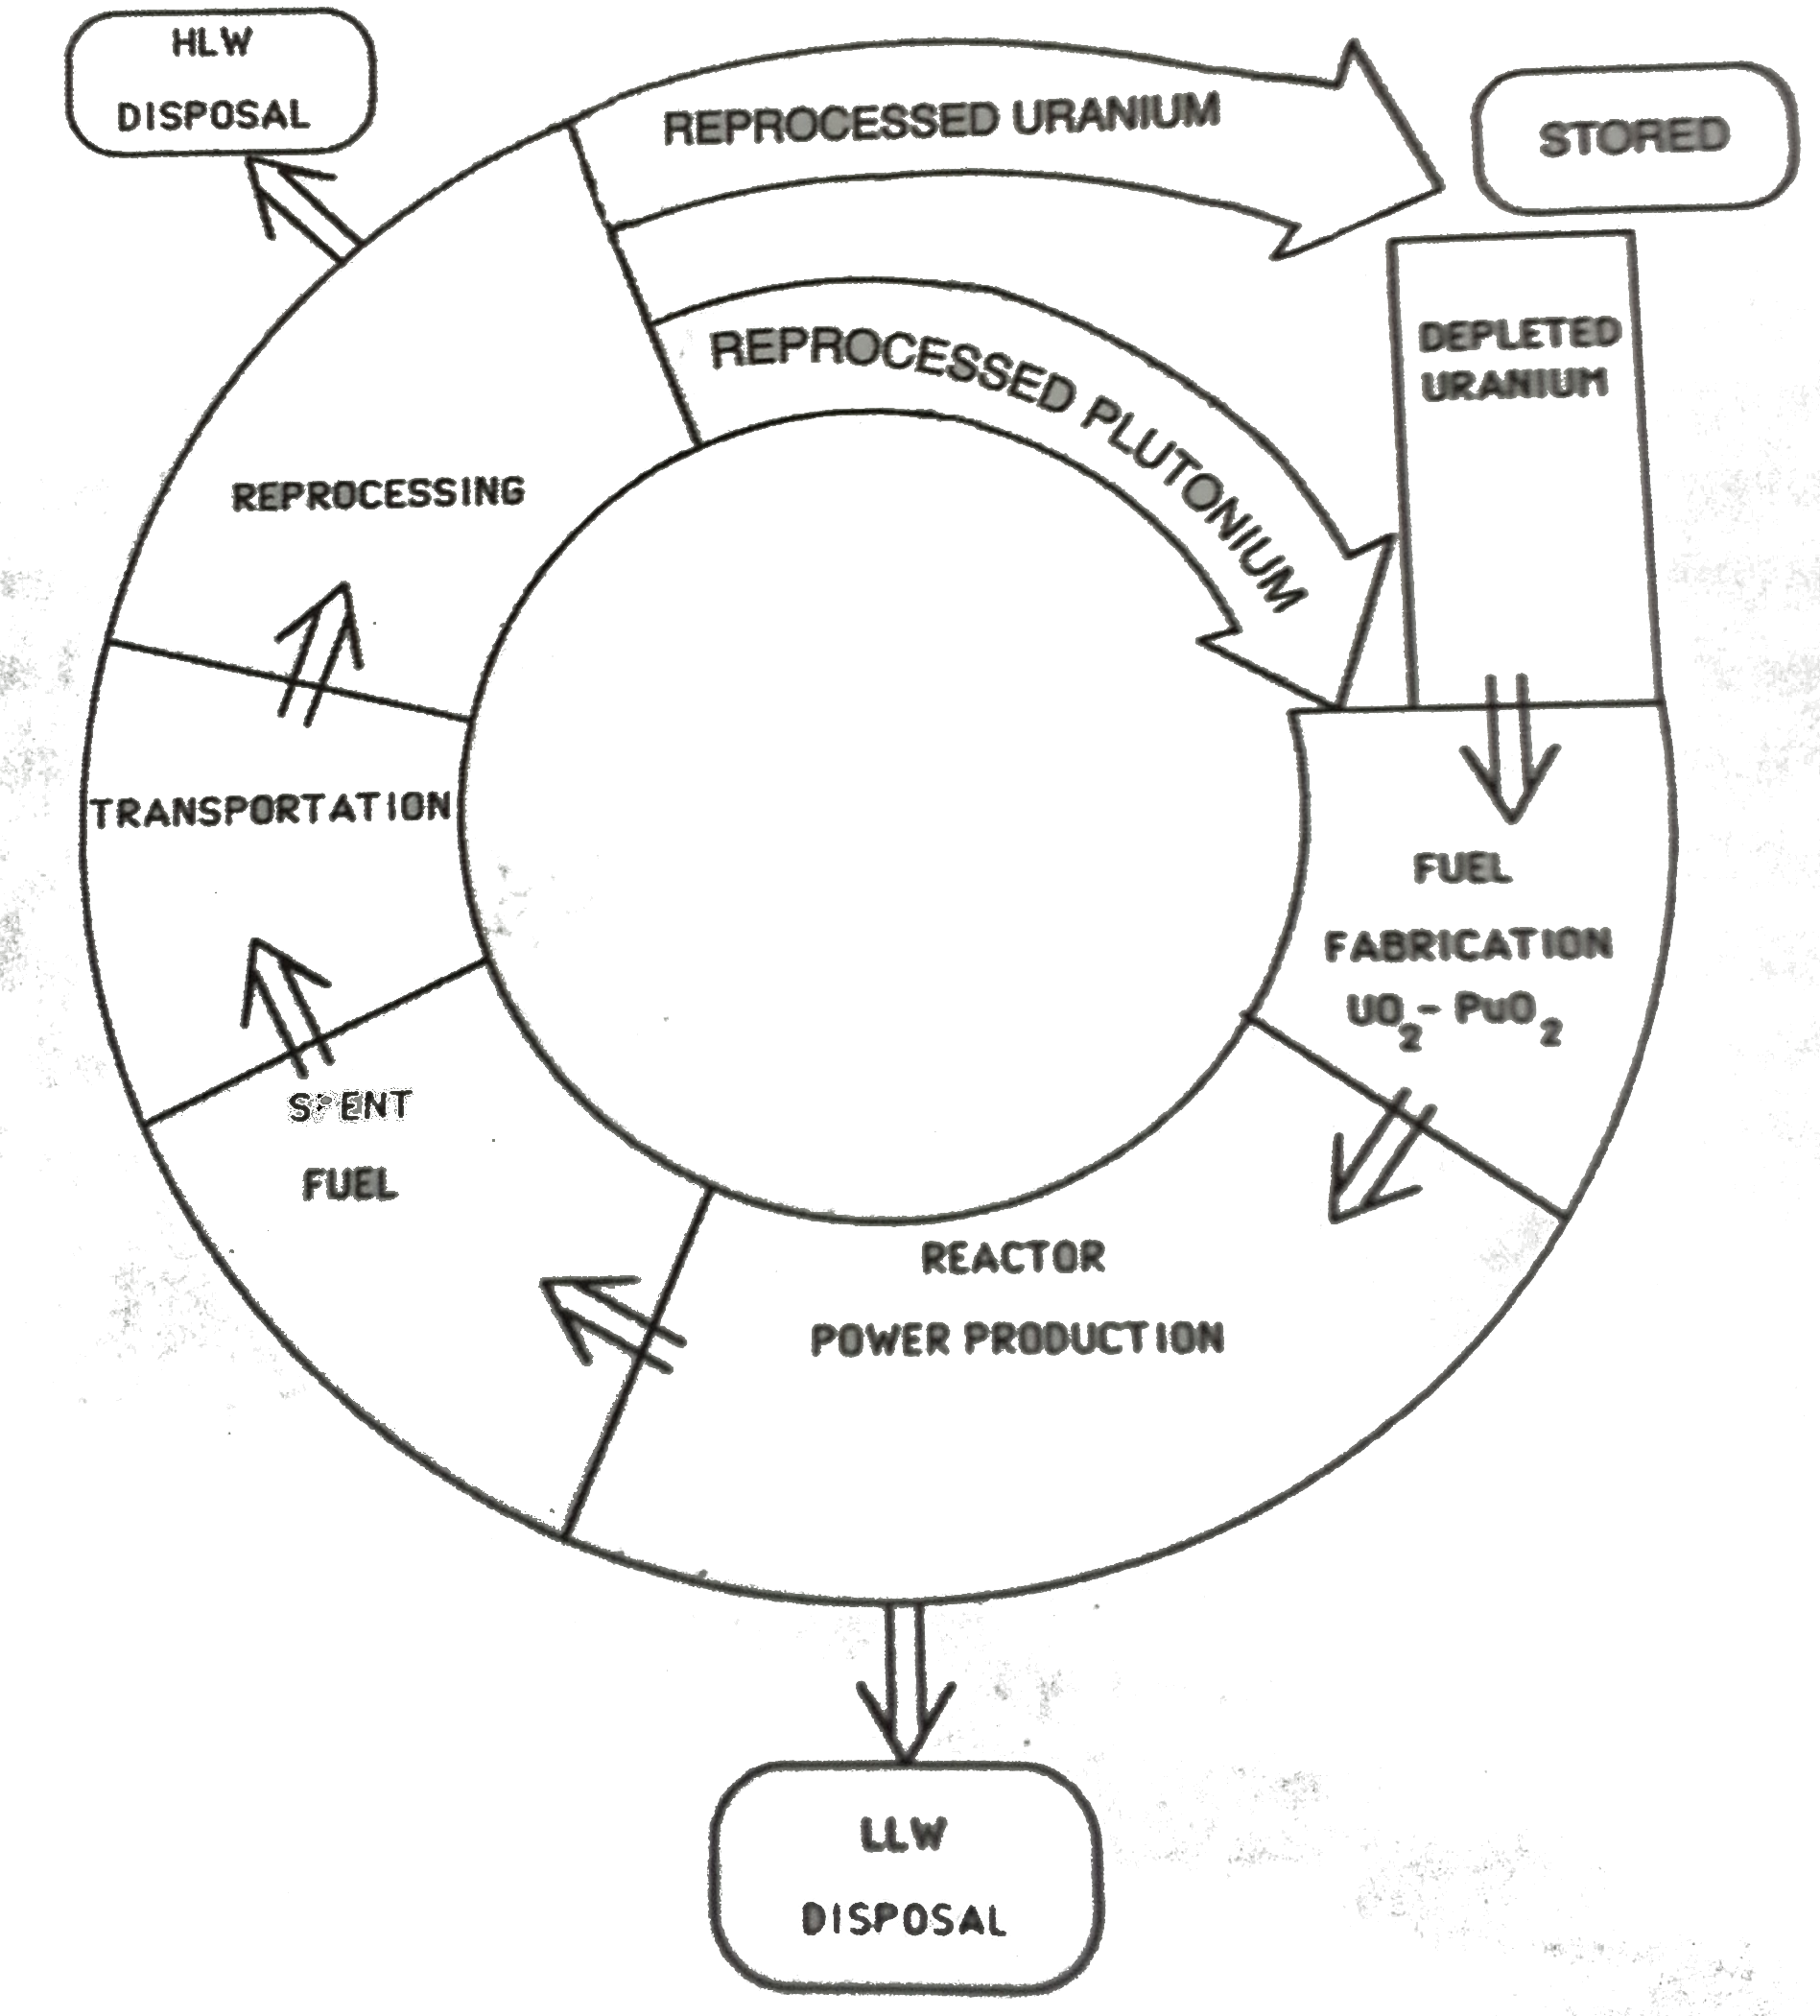
\includegraphics[height=7.5cm]{./chapters/intro/closed_cycle.png}
  \caption{The closed fuel cycle as shown in \cite{cochran1990nuclear}.}
  \label{fig:closed-cycl}e
  \end{center}
\end{figure}


The elemental groups used in fuel fabrication will depend on the fuel cycle that
is developed. The currently-operating large-scale industrial reprocessing plants
(La Hague in France, THORP in the U.K., Mayak in Russia, and Rokkasho in Japan)
utilize the PUREX process to extract uranium and plutonium. The plutonium is
then oxidized and mixed with depleted uranium from the enrichment process to
produce mixed-oxide fuel (MOX). Other sources of uranium can be used to fill MOX
fuel, such as recycled uranium from reprocessing, as neutronics-related
reactivity and safety constraints allow. Other fuel cycles utilize the mixed
actinides elemental group as well. Generally, plutonium is included with the
mixed actinides, which results in a elemental category called the transuranic
(TRU) elements. These fuel cycles generally include fast reactors that convert
their TRU inventory into either more TRU (i.e., they have a conversion ratio
(CR) of greater than 1), less TRU (CR < 1), or they maintain the amount of TRU
entering and exiting their system (CR = 1). Fast reactors with CR > 1 are termed
breeder reactors.

It should be noted that with any reprocessing capability, nonproliferation
issues arise. Nuclear weapons have historically been produced using either
enriched uranium or reprocessed plutonium; however it is possible to produce one
with any mix of appropriate materials. Accordingly, any fuel cycle that exposes
bare plutonium streams has an inherently higher nonproliferation risk than one
that does not, and such risks must be weighed accordingly. On a technical note,
though, the relatively low content of Pu-239, especially with respect to the
concentration of heat-producing Pu-240, in spent LWR fuel makes diverting such
fuel for the purposes of nuclear weaponry a route with an incredibly low
probability of success.


\subsection{The Modified-Open Fuel Cycle}
The modified open fuel cycle is effectively a hybrid of the open and closed fuel
cycles. The Blue Ribbon Commission's Reactor and Fuel Cycle
Technology Subcommittee tackled a definition as follows:

\begin{quotation}
We have defined this category to encompass a very wide range of possible fuel
cycles with multiple possible combinations of different reactor, separations,
and fuel fabrication technologies. Our definition includes any fuel cycle in
which some of the spent fuel is processed rather than being directly disposed of
after a single pass through a reactor.~\cite{brc_reactor_2012}
\end{quotation}

They mention, however, that there is no industry-wide agreed-upon
definition. For the purposes of this work I will use the committee's
definition. It should be noted that by the committee's definition, the French
nuclear power program is technically a modified-open cycle because MOX fuel
reprocessing has been demonstrated, but is not used at an industrial scale.


\section{Fuel Cycle Simulation}

\subsection{Overview}\label{sec:simulators-overview}
\input{./chapters/intro/overview}

\subsection{Metrics}
%\input{./chapters/intro/overview}

\subsection{Benchmarks}
%\input{./chapters/intro/overview}

In his conclusions of the MIT benchmarking exercise, Guerin states that
``operation of a fuel cycle model is as much art as science''
\cite{guerin_benchmark_2009}. Understanding just how much of FCS is art and how
much is science is critical to providing reliable results. 

\section{Open Questions in Fuel Cycle Simulation}

\subsection{Using Agent-Based Models}

\subsection{Input Fuel Isotopic Matching}

\subsection{Modeling Global Regions}
